\documentclass[a4paper]{article}
\usepackage[letterpaper, margin=1in]{geometry} % page format
\usepackage{listings} % this package is for including code
\usepackage{graphicx} % this package is for including figures
\usepackage{amsmath}  % this package is for math and matrices
\usepackage{amsfonts} % this package is for math fonts
\usepackage{tikz} % for drawings
\usepackage{hyperref} % for urls
\usepackage{stackengine}

\newcommand\tab[1][0.5cm]{\hspace*{#1}}

\title{Homework 1}
\author{Kaitlyn Mulligan}
\date{2/13/19}

\begin{document}
\lstset{language=Python}

\maketitle

\section{Instructions}
This assignment should be written in \LaTeX.  Please check the template that 
has been provided to you in \verb|hw.template.tar.gz| that contains the basic elements for 
you to get started.  You must show your work and how you derivated or arrived at your 
solution.  Write in understandable, easy to follow, English.\\
\tab Write all your programs in Python and make sure that your programs are included 
in your assignment.  Also include any and all figures and graphs produced using Python 
in your writeup.\\
\tab Your assignment should be submitted in two ways: through GitHub, and in hardcopy 
(in class).  You should already have a \textbf{single} repository, that will be used 
for all assignments organized in folders named "\verb|lastname-xx|", where lastname is your 
last name (or the first work of your last name if you have multiple words in it), and 
xx is the number of the assignment.  For example my GitHub folder for this assignment 
would be \verb|rivas-01| and I would put all my sources there.  Writeup: latex or word file 
(.tex/.doc), main pdf file (.pdf), and any graphics (.pdf or .eps).  Code: Python 
files (.py).


\section{Problem Set}
The following is a list of problems you will solve.  These are from your textbook.  When 
providing your solutions (hopefully using \LaTeX), do not simply give the final answer, 
show how you arrived to the solution, justify your assumptions, and explain your results 
clearly.
\begin{itemize}
    \item (extra credit) \textbf{Problem 1.2}. Use Python with matplotlib to create the 
    drawings.
    \item \textbf{Problem 1.4}. Again, use Python and the necessary packages (installed 
    for Homework 0) to do your experiments.  The purpose is for you to illustrate and shed 
    light on otherwise obscure machine learning concepts, not to produce pages and pages of 
    code.
\end{itemize}

\subsection{Problem 1.2 (extra credit)} Consider the perceptron in two dimensions: $h(\verb|x|) = \text{sign}
(\verb|w^Tx|)$ where $\verb|w| = [w_0, w_1, w_2]^{T}$ and $\verb|x| = [1, x_1, x_2]^T$.  Technically, 
$\verb|x|$ has three coordinates, but we call this perceptron two-dimensional because the first 
coordinate is fixed at $1$.
\begin{itemize}
    \item[(a)] Show that the regions on the plane where $h(x) = +1$ and $h(x) = -1$ are separated 
    by a line.  If we express this line by the equation $x_2 = ax_1 + b$, what are the slope $a$ and 
    intercept $b$ in terms of $w_0, w_1, w_2$?\\
    \textbf{Solution:} If we have $h(x) = +1$ we know that $\verb|w|^T x$ will be greater than $0$.  
    Also if we have $h(x) = -1$ we know that $\verb|w|^T x$ is less than $0$.  From this we can conclude 
    that somewhere between these two regions, there is a line who equation can be written as 
    $\verb|w|^T x = 0$ or $w_0 + w_1x_1 + w_2x_2 = 0$.  This can be rewritten as $x_2 = ax_1 + b$.  From these equations we can determine that the slope, $a$, is$a = -w_1 / w_2$ and the intercept, $b$, is $b = -w_0 / w_2$.
    \item[(b)] Draw a picture for the cases $\verb|w| = [1, 2, 3]^T$ and $\verb|w| = -[1, 2, 3]^T$.\\
    \textbf{Solution:} For $\verb|w| = [1, 2, 3]^T$ we have the following:
    \begin{center}
        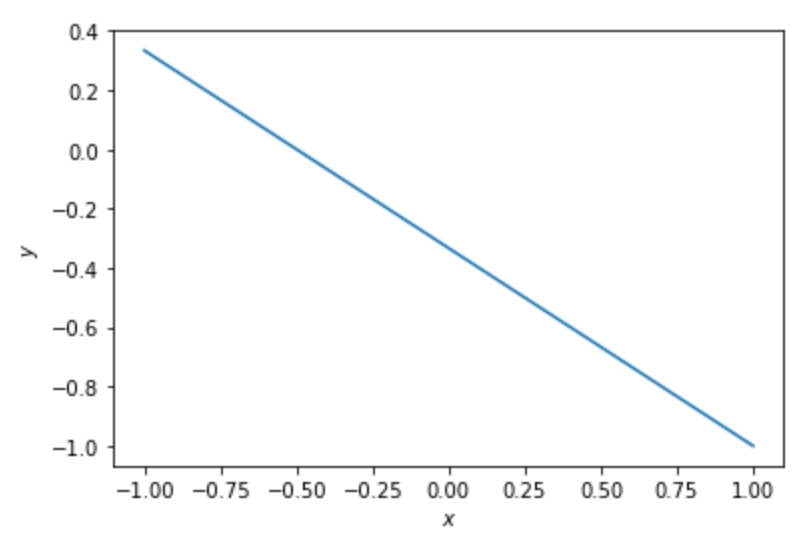
\includegraphics[width=0.6\textwidth]{1-2-b1.jpg}
    \end{center}
    For $\verb|w| = -[1, 2, 3]^T$ we have the following:
    \begin{center}
        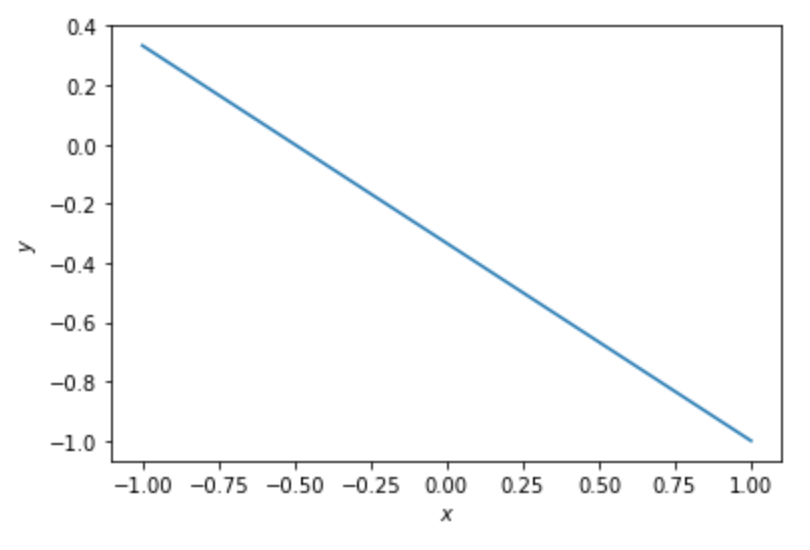
\includegraphics[width=0.6\textwidth]{1-2-b2.jpg}
    \end{center}
\end{itemize}
In more than two dimensions, the $+1$ and $-1$ regions are separated by a \textit{hyperplane}, the 
generalization of a line.

\subsection{Problem 1.4} In Exercise 1.4, we use an artificial data set to study the perceptron 
learning algorithm.  This problem leads you to explore the algorithm further with data sets of 
different sizes and dimensions.
\begin{itemize}
    \item[(a)] Generate a linearly separable data set of size 20 as indicated in Exercise 1.4.  
    Plot the examples $\{(\verb|x|_n, y_n)\}$ as well as the target function $f$ on a plane.  
    Be sure to mark the examples from different classes differently, and add labels to the axes 
    of the plot.\\
    \textbf{Solution:}
    \begin{center}
        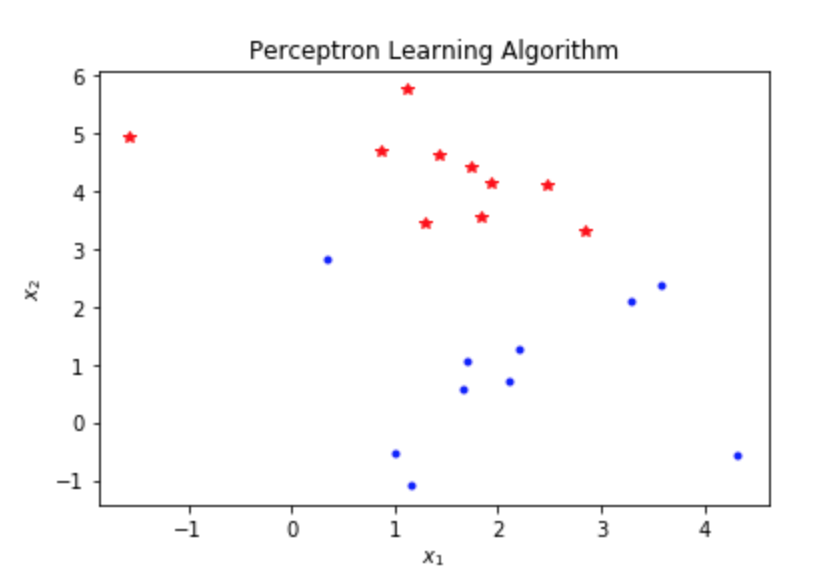
\includegraphics[width=0.6\textwidth]{1-4-a.jpg}
    \end{center}
    \item[(b)] Run the perceptron learning algorithm in the data set above.  Report the number 
    of updates that the algorithm takes before converging.  Plot the examples $\{(\verb|x|_n, y_n)\}$, 
    the target function $f$, and the final hypothesis $g$ in the same figure.  Comment on whether 
    $f$ is close to $g$.\\
    \textbf{Solution:} The algorithm took 30 iterations before converging.
    \begin{center}
        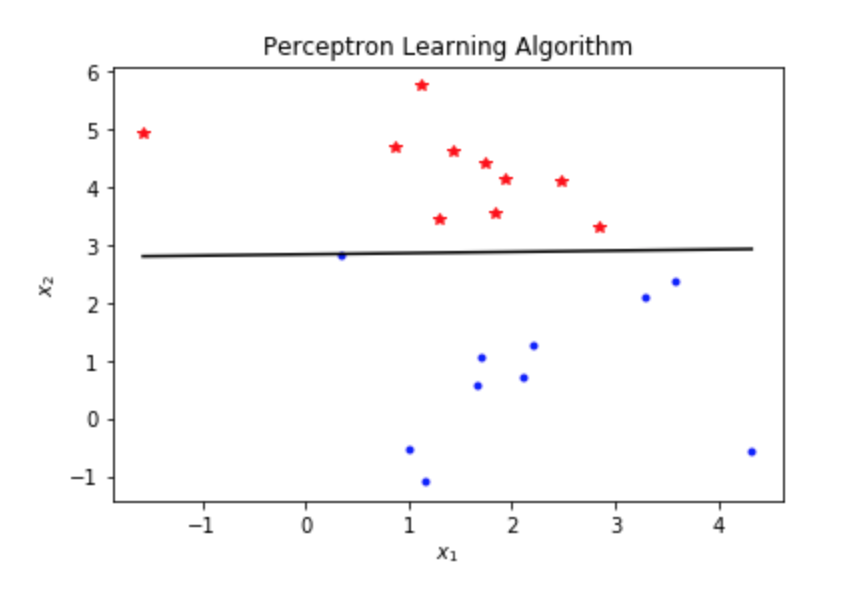
\includegraphics[width=0.6\textwidth]{1-4-b.jpg}
    \end{center}
    \item[(c)] Repeat everything in (b) with another randomly generated data set of size 20.  
    Compare your results with (b).\\
    \textbf{Solution:} With another randomly generated data set of size 20, the algorithm only 
    took 2 iterations to converge.  This data set took a lot less number of iterations than the 
    previous data set.  Looking at the graph, we can see this data was originally grouped together, 
    which allowed the algorithm to converge faster.
    \begin{center}
        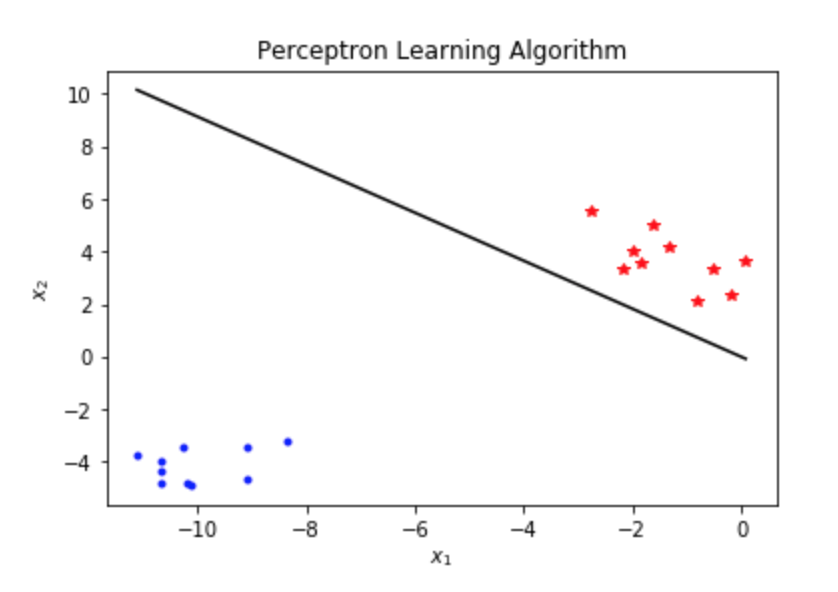
\includegraphics[width=0.6\textwidth]{1-4-c.jpg}
    \end{center}
    \item[(d)] Repeat everything in (b) with another randomly generated data set of size 100.  
    Compare your results with (b).\\
    \textbf{Solution:} With a randomly generated data set of size 100, the algorithm was able to 
    converge in 27 iterations.  Compared to part (b), the algorithm took less iterations to converge, 
    but this data was grouped better than it was in part (b).
    \begin{center}
        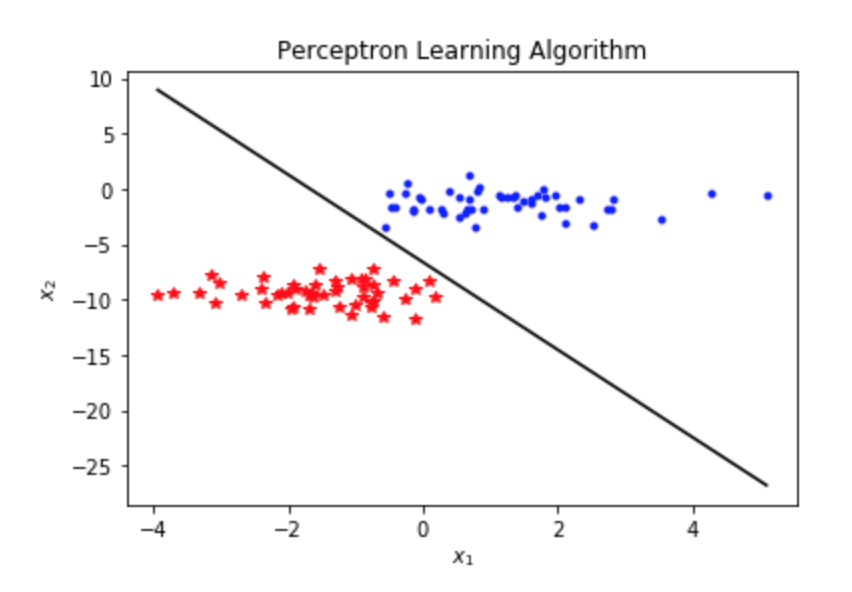
\includegraphics[width=0.6\textwidth]{1-4-d.jpg}
    \end{center}
    \item[(e)] Repeat everything in (b) with another randomly generated data set of size 1000.  
    Compare your results with (b).\\
    \textbf{Solution:} With a randomly generated data set of size 1000, the algorithm converged in 
    298 iterations.
    \begin{center}
        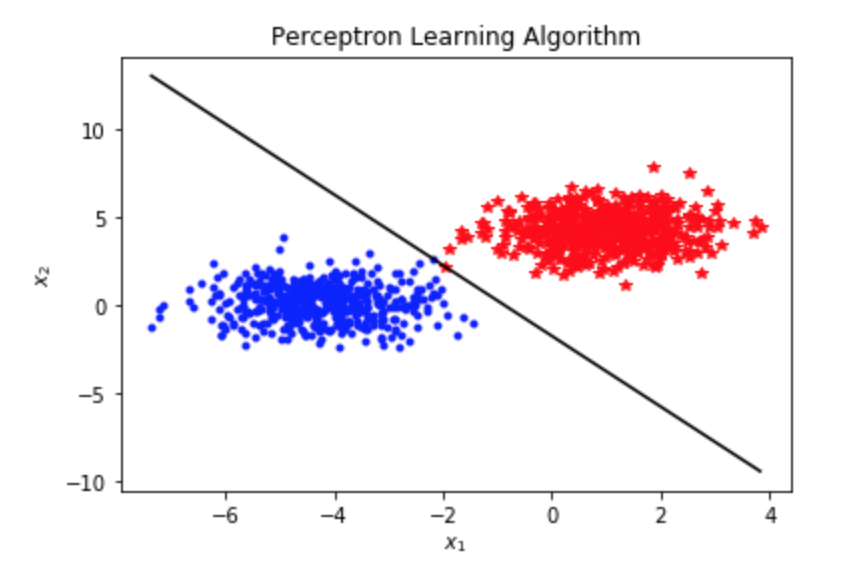
\includegraphics[width=0.6\textwidth]{1-4-e.jpg}
    \end{center}
    \item[(f)] Modify the algorithm such that it takes $\verb|x|_n \in \mathbb{R}^{10}$ instead 
    of $\mathbb{R}^2$.  Randomly generate a linearly separable data set of size 1000 with 
    $\verb|x|_n \in \mathbb{R}^{10}$ and feed the data set to the algorithm.  How many updates 
    does the algorithm take to converge?\\
    \textbf{Solution:} After modifying the algorithm, a randomly generated data set of size 1000, 
    with $\verb|x|_n \in \mathbb{R}^{10}$, the algorithm was able to converge in 2 iterations.
    \item[(g)] Repeat the algorithm on the same data set as (f) for 100 experiments.  In the 
    iterations of each experiment, pick $\verb|x|(t)$ randomly instead of deterministically.  
    Plot a histogram for the number of updates that the algorithm takes to converge.\\
    \textbf{Solution:} After repeating the algorithm on the same data set as part (f) for 100 
    experiments, below is a histogram to show the count of number of iterations each experiment 
    took to converge.  As can be seen, it looks to be around 30 experiments took 1 iteration and 
    around 70 experiments took 2 iterations.
    \begin{center}
        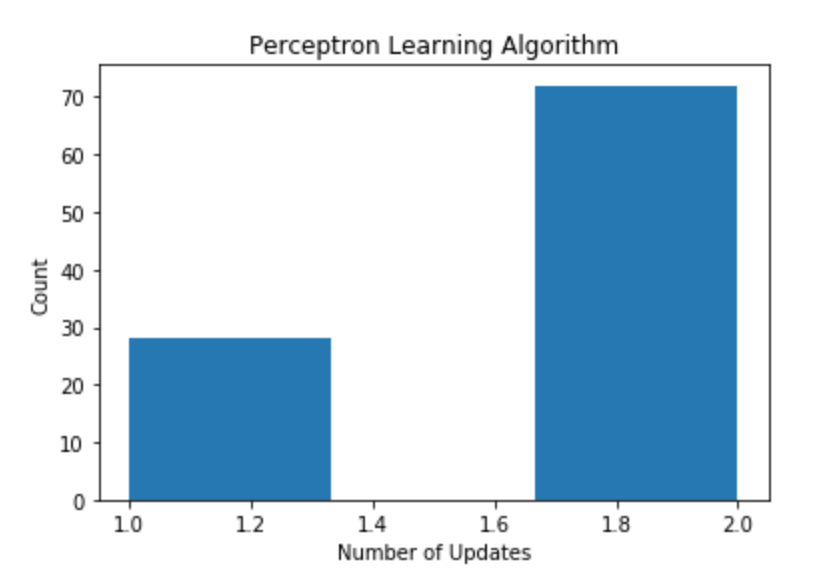
\includegraphics[width=0.6\textwidth]{1-4-g.jpg}
    \end{center}
    \item[(h)] Summarize your conclusions with respect to accuracy and running time as a 
    function of $N$ and $d$.
    \textbf{Solution:} After running all of these experiments with different data sets and 
    different sizes of the data sets, it seems that the bigger data sets (increasing N) will 
    give you a better approximation, but also cause it to take more time to run.  Also the 
    bigger d is, the greater the running time will become.
\end{itemize}

\end{document}
